% XeLaTeX

\documentclass{article}
\usepackage{ctex}
\usepackage{xypic}
\usepackage{amsfonts,amssymb}
\usepackage{multirow}
\usepackage{geometry}
\usepackage{graphicx}
\usepackage{listings}
\usepackage{lipsum}
\usepackage{courier}
\usepackage{fancyvrb}
\usepackage{etoolbox}


\linespread{1.2}
\geometry{left=3cm,right=2.5cm,top=2.5cm,bottom=2.5cm}

\makeatletter
\patchcmd{\FV@SetupFont}
  {\FV@BaseLineStretch}
  {\fontencoding{T1}\FV@BaseLineStretch}
  {}{}
\makeatother

\lstset{basicstyle=\small\fontencoding{T1}\ttfamily,breaklines=true}
\lstset{numbers=left,frame=shadowbox,tabsize=4}
%\lstset{extendedchars=false}
\begin{document}

\title{实验四 \text{ } verilog 数字系统设计基础 \text{ } 实验报告}
\author {16337233 王凯祺}
\maketitle

\section{实验目的}

1. 掌握 verilog 数字系统设计语言

2. 能使用 verilog 数字系统设计出一个简单的全减器

\section{实验原理}

1. 列出全减器真值表

2. 由真值表写函数式

3. 对函数式进行化简

4. 使用结构化描述的建模方式、数据流描述的建模方式、行为描述的建模方式为全减器建模,完成一个全减器的 verilog 设计

\section{实验仪器}

Vivado 2015.3
Basys 3 实验板

\section{实验内容}

使用结构化描述的建模方式、数据流描述的建模方式、行为描述的建模方式为全减器建模,完成一个全减器的 verilog 设计

\newpage

\section{实验设计}

\subsection{真值表}

\begin{table}[!hbp]
\centering
\begin{tabular}{|c|c|c||c|c|}
\hline
a & b & cin & sum & cout \\
\hline
\hline
0 & 0 & 0 & 0 & 0 \\
\hline
0 & 0 & 1 & 1 & 1 \\
\hline
0 & 1 & 0 & 1 & 1 \\
\hline
0 & 1 & 1 & 0 & 1 \\
\hline
1 & 0 & 0 & 1 & 0 \\
\hline
1 & 0 & 1 & 0 & 0 \\
\hline
1 & 1 & 0 & 0 & 0 \\
\hline
1 & 1 & 1 & 1 & 1 \\
\hline

\end{tabular}
\end{table}


\subsection{表达式}

$sum = (\overline{a} \& \overline{b} \& cin) \| (\overline{a} \& b \& \overline{cin}) \| (a \& \overline{b} \& \overline{cin}) \| (a \& b \& cin) = a \oplus b \oplus cin$

$cout = (\overline{a} \& \overline{b} \& cin) \| (\overline{a} \& b \& \overline{cin}) \| (\overline{a} \& b \& cin) \| (a \& b \& cin) = (\overline{a} \& b) \| (\overline{a} \& cin) \| (b \& cin)$

\subsection{建模}

\subsubsection{结构化描述的建模方式}

\begin{lstlisting}
module minus_1(input a, input b, input cin, output sum, output cout);
    wire s1, t1, t2, t3, na;
    xor x1(s1, a, b);
    xor x2(sum, s1, cin);
    not n1(na, a);
    and a1(t1, na, b);
    and a2(t2, na, cin);
    and a3(t3, b, cin);
    or o1(cout, t1, t2, t3);
endmodule
\end{lstlisting}

\subsubsection{数据流描述的建模方式}

\begin{lstlisting}
module minus_2(input a, input b, input cin, output sum, output cout);
    wire s1, t1, t2, t3, na;
    assign s1 = a ^ b;
    assign sum = s1 ^ cin;
    assign na = ~a;
    assign t1 = na & b;
    assign t2 = na & cin;
    assign t3 = b & cin;
    assign cout = t1 | t2 | t3;
endmodule
\end{lstlisting}

\subsubsection{行为描述的建模方式}

\begin{lstlisting}
module minus_3(input a, input b, input cin, output sum, output cout);
    reg sum;
    reg cout;
    always @ (a or b or cin) begin
        sum = a ^ b ^ cin;
        cout = (~a & b) | (~a & cin) | (b & cin);
    end
endmodule
\end{lstlisting}

\subsubsection{仿真文件}

\begin{lstlisting}
module minus_tb();
    reg a;
    reg b;
    reg cin;    
    wire sum1, sum2, sum3;
    wire cout1, cout2, cout3;    
    minus_1 uut1(.a(a), .b(b), .cin(cin), .sum(sum1), .cout(cout1));
    minus_2 uut2(.a(a), .b(b), .cin(cin), .sum(sum2), .cout(cout2));
    minus_3 uut3(.a(a), .b(b), .cin(cin), .sum(sum3), .cout(cout3));
    initial begin
        a = 0;
        b = 0;
        cin = 0;
        #2;
    end    
    integer i, j;
    always begin
        for (i = 0; i < 8; i = i + 1) begin
            j = i;
            cin = j & 1;
            j = j >> 1;
            b = j & 1;
            j = j >> 1;
            a = j & 1;
            #2;
        end
    end
endmodule
\end{lstlisting}

\newpage

\subsubsection{仿真波形图}

\begin{figure}[!hbp]
  \centering
  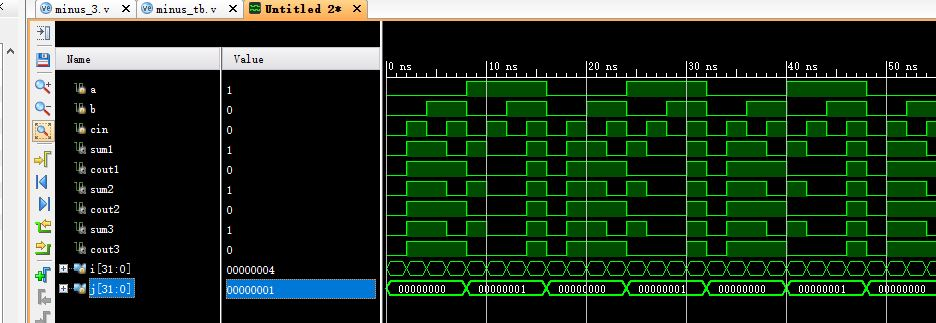
\includegraphics[scale=0.6]{s1.jpg}
\end{figure}


\end{document}
















